\documentclass[10pt,a4paper]{article}
\usepackage[margin=2.2cm]{geometry}
\usepackage{fontspec}
\usepackage{kotex}
\setmainfont{Apple SD Gothic Neo}
\setsansfont{Apple SD Gothic Neo}
\usepackage{amsmath,amssymb}
\usepackage{graphicx}
\usepackage{booktabs}
\usepackage{caption}
\usepackage[dvipsnames]{xcolor}
\usepackage[colorlinks=true,linkcolor=MidnightBlue,citecolor=MidnightBlue,
            urlcolor=MidnightBlue]{hyperref}
\usepackage{titlesec}
\titleformat{\section}{\large\bfseries}{\thesection}{0.6em}{}
\captionsetup{font=small,labelfont=bf}
\setlength{\parskip}{0.35em}
\setlength{\parindent}{0pt}

\usepackage{mdframed}
\newmdenv[linewidth=0.4pt,linecolor=gray!60,backgroundcolor=gray!5,
          innertopmargin=6pt,innerbottommargin=6pt,skipabove=8pt,skipbelow=8pt]{claimbox}
\newcommand{\claim}[2]{\begin{claimbox}\textbf{주장.} #1\par\smallskip
  \textcolor{gray!70}{\textbf{반증 조건.} #2}\end{claimbox}}

\title{\bfseries 릿지 한 줄\\[2pt]
\large 경쟁 베이스라인이 도착했다 --- 그리고 전이를 이겼다}
\author{월드모델 실험실 · 노트 $821$}
\date{2026-08-07}
\begin{document}\maketitle

\section{한 줄}

사용자 지적 ②를 이행했다 --- \emph{``$\rho\,0.30$ 이 좋은지 나쁜지 비교 대상이
없다. 단순 방법이 $0.25$ 를 내면 사실상 $0$ 이다.''} 논문 $178$ 과 같은
자(KR 만화 · 평가 $=2025{\sim}26$ 시작 $322$행 · 풀 $=$ 과거 $1{,}394$행)에서
단순 방법 넷을 쟀다.

\begin{center}
\begin{tabular}{lrl}
\toprule
방법 & 평가 $\rho$ & \\
\midrule
분기 평균 사상 & $-0.130$ & 풀에서만 학습 \\
시작일 순위(최근성) & $-0.099$ & \\
target\_breadth 단독(사전 지정) & $+0.008$ & 예측 빗나감 \\
챔피언 전이(자료 $0$건) & $+0.2958$ & 논문 $178$ \\
TabPFN $800$건 단독 & $+0.3383$ & 논문 $178$ \\
\textbf{릿지 한 줄(풀 $1{,}394$)} & $\mathbf{+0.3393}$ & \textbf{위약 $-0.023$} \\
\bottomrule
\end{tabular}
\end{center}

\textbf{판정: 갈래 $2$ --- 베이스라인 승.} 그리고 문턱($0.25$)을 넘은 정도가
아니라 \textbf{전이를 $+0.0435$(KR $2\sigma$ 의 $1.7$배)로 이긴다.}

\begin{figure}[t]\centering
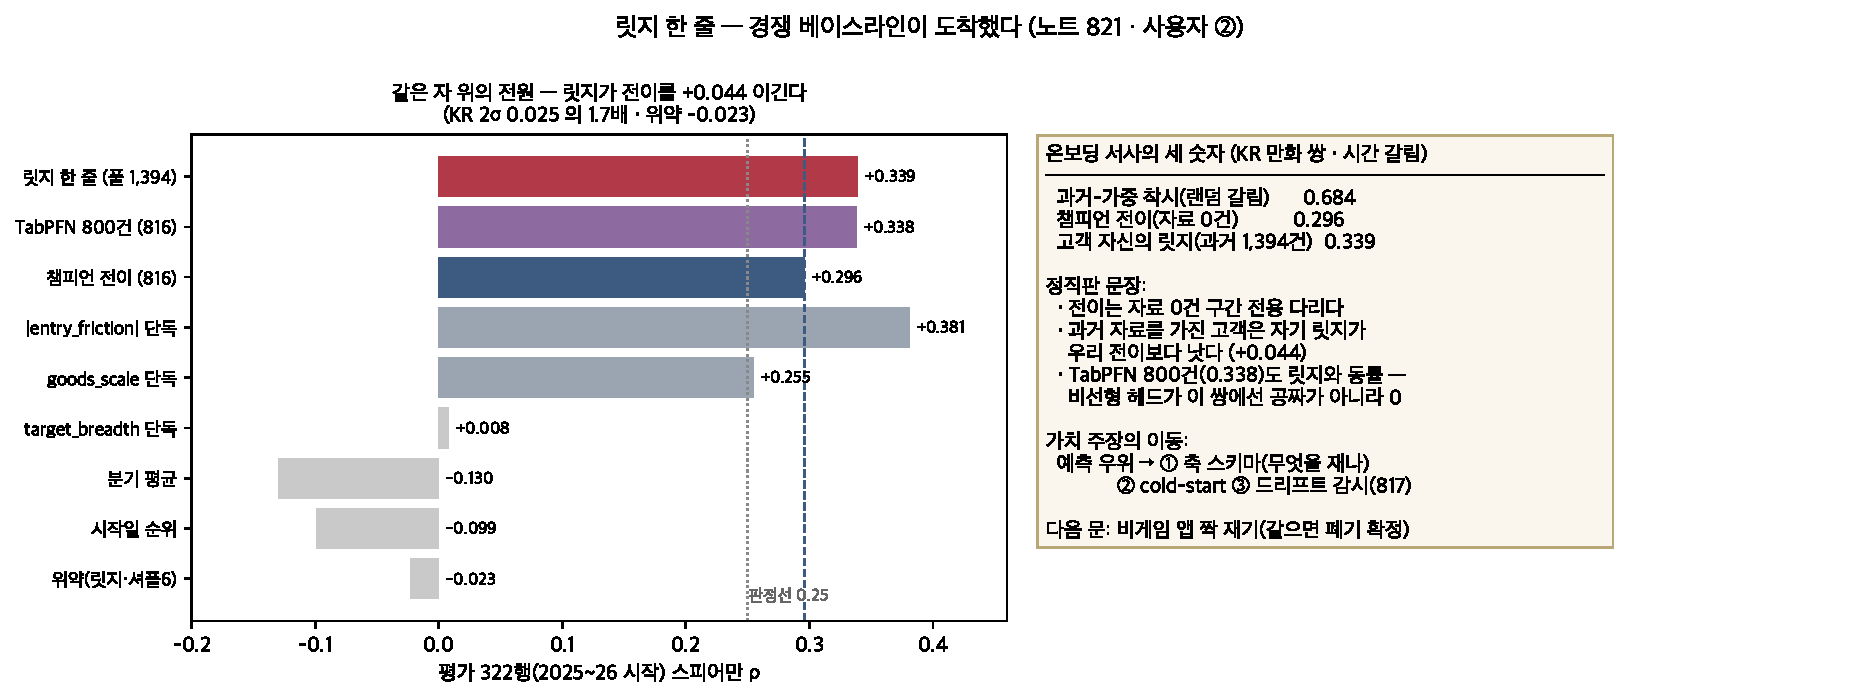
\includegraphics[width=0.97\textwidth]{figs/ridge.pdf}
\caption{왼쪽: 같은 자 위의 전원. 오른쪽: 온보딩 서사의 세 숫자와 정직판.}
\end{figure}

\section{무엇이 죽고 무엇이 남나}

\claim{\textbf{`$50$건이면 전이와 동급' 온보딩 서사는 이 쌍에서 폐기된다.}
과거 자료를 가진 고객은 자기 릿지 한 줄($5$축$+$마스크$+t$ · $\alpha{=}1$)이
우리 전이보다 낫다. 덤으로 \textbf{TabPFN $800$건($0.3383$)과 릿지($0.3393$)가
동률} --- 이 쌍에선 비선형 헤드도 릿지 위에 아무것도 안 얹는다. $t$ 열을 빼도
$0.3298$ 이라 신호는 시간 추세가 아니라 축이고, 릿지 계수는 target\_breadth
$+1.40$ · goods\_scale $+1.11$ · entry\_friction $-0.41$(부호 반전을 스스로
처리 --- 단독 축 $|\rho|$ 최강 $-0.381$ 은 BagBoost OOC\_DROP 주석의 `KR 짝 안
부호 $-0.320$' 의 실물 재확인이다). 풀 안 CV $0.686$ 대 평가 $0.339$ ---
반토막은 방법이 아니라 \textbf{시간의 성질}이다(논문 $178$ 재확인).}
{\textbf{가치 주장의 이동}: 예측 우위 $\to$ ① 축 스키마(무엇을 재야 하는지 ---
릿지의 재료 자체가 우리 축이다) ② cold-start(자료 $0$건 다리) ③ 드리프트
감시($817$ · 도메인마다 닳는 속도). 판정은 KR 쌍 하나 --- \textbf{비게임 앱
짝에서 같은 릿지}가 다음이고(같으면 폐기 확정 · 갈리면 쌍 특유), 판 안
도메인들의 합동 대 도메인별 릿지 비교가 그 다음이다. 판 $\rho$ $0.4689$ 그대로.}

\end{document}
